%CUT AND PASTE THIS ENTIRE DOCUMENT INTO A BLANK DOCUMENT ON CloudSageMath. Then replace the content (title, name, and so on), with your stuff. If you have problems or errors, let me know! 

%\documentclass[12pt]{amsart}
\documentclass{article}

\usepackage{tikz-cd}

%Python Code Listing
\usepackage[utf8]{inputenc}
\usepackage[english]{babel}
\usepackage[T1]{fontenc}

\usepackage{xcolor}
\definecolor{maroon}{cmyk}{0, 0.87, 0.68, 0.32}
\definecolor{halfgray}{gray}{0.55}
\definecolor{ipython_frame}{RGB}{207, 207, 207}
\definecolor{ipython_bg}{RGB}{247, 247, 247}
\definecolor{ipython_red}{RGB}{186, 33, 33}
\definecolor{ipython_green}{RGB}{0, 128, 0}
\definecolor{ipython_cyan}{RGB}{64, 128, 128}
\definecolor{ipython_purple}{RGB}{170, 34, 255}



\usepackage{listings}
\lstset{
    breaklines=true,
    %
    extendedchars=true,
    literate=
    {á}{{\'a}}1 {é}{{\'e}}1 {í}{{\'i}}1 {ó}{{\'o}}1 {ú}{{\'u}}1
    {Á}{{\'A}}1 {É}{{\'E}}1 {Í}{{\'I}}1 {Ó}{{\'O}}1 {Ú}{{\'U}}1
    {à}{{\`a}}1 {è}{{\`e}}1 {ì}{{\`i}}1 {ò}{{\`o}}1 {ù}{{\`u}}1
    {À}{{\`A}}1 {È}{{\'E}}1 {Ì}{{\`I}}1 {Ò}{{\`O}}1 {Ù}{{\`U}}1
    {ä}{{\"a}}1 {ë}{{\"e}}1 {ï}{{\"i}}1 {ö}{{\"o}}1 {ü}{{\"u}}1
    {Ä}{{\"A}}1 {Ë}{{\"E}}1 {Ï}{{\"I}}1 {Ö}{{\"O}}1 {Ü}{{\"U}}1
    {â}{{\^a}}1 {ê}{{\^e}}1 {î}{{\^i}}1 {ô}{{\^o}}1 {û}{{\^u}}1
    { }{{\^A}}1 {Ê}{{\^E}}1 {Î}{{\^I}}1 {Ô}{{\^O}}1 {Û}{{\^U}}1
    {œ}{{\oe}}1 {Œ}{{\OE}}1 {æ}{{\ae}}1 {Æ}{{\AE}}1 {ß}{{\ss}}1
    {ç}{{\c c}}1 {Ç}{{\c C}}1 {ø}{{\o}}1 {å}{{\r a}}1 {Å}{{\r A}}1
    {€}{{\EUR}}1 {£}{{\pounds}}1
}

%%
%% Python definition (c) 1998 Michael Weber
%% Additional definitions (2013) Alexis Dimitriadis
%% modified by me (should not have empty lines)
%%
\lstdefinelanguage{iPython}{
    morekeywords={access,and,break,class,continue,def,del,elif,else,except,exec,finally,for,from,global,if,import,in,is,lambda,not,or,pass,print,raise,return,try,while},%
    %
    % Built-ins
    morekeywords=[2]{abs,all,any,basestring,bin,bool,bytearray,callable,chr,classmethod,cmp,compile,complex,delattr,dict,dir,divmod,enumerate,eval,execfile,file,filter,float,format,frozenset,getattr,globals,hasattr,hash,help,hex,id,input,int,isinstance,issubclass,iter,len,list,locals,long,map,max,memoryview,min,next,object,oct,open,ord,pow,property,range,raw_input,reduce,reload,repr,reversed,round,set,setattr,slice,sorted,staticmethod,str,sum,super,tuple,type,unichr,unicode,vars,xrange,zip,apply,buffer,coerce,intern},%
    %
    sensitive=true,%
    morecomment=[l]\#,%
    morestring=[b]',%
    morestring=[b]",%
    %
    morestring=[s]{'''}{'''},% used for documentation text (mulitiline strings)
    morestring=[s]{"""}{"""},% added by Philipp Matthias Hahn
    %
    morestring=[s]{r'}{'},% `raw' strings
    morestring=[s]{r"}{"},%
    morestring=[s]{r'''}{'''},%
    morestring=[s]{r"""}{"""},%
    morestring=[s]{u'}{'},% unicode strings
    morestring=[s]{u"}{"},%
    morestring=[s]{u'''}{'''},%
    morestring=[s]{u"""}{"""},%
    %
    % {replace}{replacement}{lenght of replace}
    % *{-}{-}{1} will not replace in comments and so on
    literate=
    {á}{{\'a}}1 {é}{{\'e}}1 {í}{{\'i}}1 {ó}{{\'o}}1 {ú}{{\'u}}1
    {Á}{{\'A}}1 {É}{{\'E}}1 {Í}{{\'I}}1 {Ó}{{\'O}}1 {Ú}{{\'U}}1
    {à}{{\`a}}1 {è}{{\`e}}1 {ì}{{\`i}}1 {ò}{{\`o}}1 {ù}{{\`u}}1
    {À}{{\`A}}1 {È}{{\'E}}1 {Ì}{{\`I}}1 {Ò}{{\`O}}1 {Ù}{{\`U}}1
    {ä}{{\"a}}1 {ë}{{\"e}}1 {ï}{{\"i}}1 {ö}{{\"o}}1 {ü}{{\"u}}1
    {Ä}{{\"A}}1 {Ë}{{\"E}}1 {Ï}{{\"I}}1 {Ö}{{\"O}}1 {Ü}{{\"U}}1
    {â}{{\^a}}1 {ê}{{\^e}}1 {î}{{\^i}}1 {ô}{{\^o}}1 {û}{{\^u}}1
    { }{{\^A}}1 {Ê}{{\^E}}1 {Î}{{\^I}}1 {Ô}{{\^O}}1 {Û}{{\^U}}1
    {œ}{{\oe}}1 {Œ}{{\OE}}1 {æ}{{\ae}}1 {Æ}{{\AE}}1 {ß}{{\ss}}1
    {ç}{{\c c}}1 {Ç}{{\c C}}1 {ø}{{\o}}1 {å}{{\r a}}1 {Å}{{\r A}}1
    {€}{{\EUR}}1 {£}{{\pounds}}1
    %
    {^}{{{\color{ipython_purple}\^{}}}}1
    {=}{{{\color{ipython_purple}=}}}1
    %
    {+}{{{\color{ipython_purple}+}}}1
    {*}{{{\color{ipython_purple}$^\ast$}}}1
    {/}{{{\color{ipython_purple}/}}}1
    %
    {+=}{{{+=}}}1
    {-=}{{{-=}}}1
    {*=}{{{$^\ast$=}}}1
    {/=}{{{/=}}}1,
    literate=
    *{-}{{{\color{ipython_purple}-}}}1
     {?}{{{\color{ipython_purple}?}}}1,
    %
    identifierstyle=\color{black}\ttfamily,
    commentstyle=\color{ipython_cyan}\ttfamily,
    stringstyle=\color{ipython_red}\ttfamily,
    keepspaces=true,
    showspaces=false,
    showstringspaces=false,
    %
    rulecolor=\color{ipython_frame},
    frame=single,
    frameround={t}{t}{t}{t},
    framexleftmargin=6mm,
    numbers=left,
    numberstyle=\tiny\color{halfgray},
    %
    %
    backgroundcolor=\color{ipython_bg},
    %   extendedchars=true,
    basicstyle=\scriptsize,
    keywordstyle=\color{ipython_green}\ttfamily,
}

%%%%flowchart
\usetikzlibrary{shapes.geometric, arrows}
\tikzstyle{startstop} = [rectangle, rounded corners, minimum width=3cm, minimum height=1cm, text width=25em,text centered, draw=black, fill=yellow!30]
\tikzstyle{io} = [trapezium, trapezium left angle=70, trapezium right angle=110, minimum width=3cm, minimum height=1cm, text centered, draw=black, fill=blue!30]
\tikzstyle{process} = [rectangle, minimum width=3cm, minimum height=1cm, text width=15em, text centered, draw=black, fill=orange!30]
%\tikzstyle{decision} = [diamond, minimum width=3cm, minimum height=1cm, text centered, draw=black, fill=green!30]
\tikzstyle{arrow} = [thick,->,>=stealth]

\tikzstyle{decision} = [rectangle, rounded corners, draw, fill=blue!20, 
    text width=15em, text badly centered, node distance=2.2cm, inner sep=0pt]
\tikzstyle{block} = [rectangle, draw, fill=blue!20, 
    text width=5em, text centered, rounded corners, minimum height=4em]
\tikzstyle{line} = [draw, -latex']
\tikzstyle{cloud} = [draw, ellipse,fill=red!20, node distance=3cm,
    minimum height=2em]
%\usepackage[english]{babel}
%\usepackage[utf8]{inputenc}
%\usepackage[margin=1in]{geometry}
%\usepackage[titletoc,title]{appendix}
\usepackage{array}
\usepackage{amsmath,amsfonts,amssymb,mathtools}
\usepackage{amsthm}
%These commands deal with theorem-like environments (i.e., italic)
\theoremstyle{plain}
%\newtheorem{theorem}{Theorem}
%\newtheorem{proposition}{Proposition}
%\newtheorem{corollary}{Corollary}
\newtheorem{property}{Property}
%\newtheorem{definition}{Definition}
%\newtheorem{proof}{Proof}
%\newtheorem{lemma}{Lemma}
%\newtheorem{claim}{Claim}
%\newtheorem{example}{Example}
\newtheorem{non-example}{Non-Example}

\DeclareMathOperator{\id}{id}
\DeclareMathOperator{\Tr}{Tr}


\usepackage{hyperref}

\usepackage{graphicx}
\usepackage{tikz,lipsum,lmodern}
\usepackage[most]{tcolorbox}

%\thispagestyle{empty}

%%%%%%from math 729

\usepackage[]{algorithm2e}
\usepackage{graphicx,float}
\usepackage{tikz}
\usetikzlibrary{graphs,graphs.standard,quotes}
\usepackage{multicol}
\usepackage{capt-of}

\usepackage{amscd,amsthm,amsmath,amssymb,amsfonts,latexsym,
graphicx,enumerate,setspace,verbatim,tocloft,rotating}
%\usepackage{color}                    % For creating colored text and background
%\usepackage{hyperref}                 % For creating hyperlinks in cross references
% other possibly useful packages: textcomp,mathrsfs,amscd,epsfig,euscript,cancel

%%%%% Layout
% These numbers might depend on your printer. Check the margins and compare them to the Graduate Division's
% guidelines. If there's something off, try playing with the numbers...
%
% For chapters:
%     Must have a minimum of 1.5in margin on left and 1in on all other sides.  Where there are page numbers
%     (whether on top or bottom), must have one additional inch between the page number and the text, for a
%     total of 2in between the edge of the paper and the text.
% For frontmatter pages:
%     The same margin numbers generally work, except for the Title Page, so you will notice that we use
%     some numbers for \textheight and \footskip right here, and then change them below, right after
%     generating the Title Page.

\hoffset=.5in 
\oddsidemargin=0in   % = 1in because LaTeX adds 1in
\evensidemargin=0in  % = 1in because LaTeX adds 1in
\topmargin=0in       % = 1in because LaTeX adds 1in
\headheight=0in
\headsep=1in         % Distance from top of pagenum (for page numbers at top-right corner of page) to text
\footskip=1.2in      % Distance from bottom of text to the page number (for page number at bottom of page)
\textwidth=5.9in     % Should be 6in, but use 5.9in to be conservative
\textheight=8.0in    % Best for Title Page (will change after the Title Page)

\pagestyle{plain}

\doublespacing

%%%%% Style of theorems, definitions, examples, equations, etc.

\theoremstyle{plain} % Heading is bold, text italic.
%\newtheorem{theorem}{Theorem}[chapter]
%\newtheorem{lemma}[theorem]{Lemma}
\newtheorem{proposition}{Proposition}
%\newtheorem{corollary}[theorem]{Corollary}
%\newtheorem{conjecture}{Conjecture}[chapter]
\newtheorem*{utheorem}{Theorem}
\newtheorem*{ucorollary}{Corollary}
\newtheorem{theorem}{Theorem}
\newtheorem{lemma}{Lemma}
\newtheorem*{ulemma}{Lemma}
\newtheorem{definition}[theorem]{Definition}

\theoremstyle{definition}  % Heading is bold, text is roman
%\newtheorem{definition}{Definition}[chapter]
%\newtheorem{example}{Example}[chapter]

\theoremstyle{remark}  % Heading is italic, text is roman
\newtheorem*{remark}{Remark}
\newtheorem*{note}{Note}
%\newtheorem{claim}{Claim}[chapter]

% Shortcuts (add your own...):
\newcommand{\N}{\mathbb{N}}
\newcommand{\Z}{\mathbb{Z}}
\newcommand{\Q}{\mathbb{Q}}
\newcommand{\R}{\mathbb{R}}
\newcommand{\C}{\mathbb{C}}
\newcommand{\e}[1]{{\mathbb E}\left[ #1 \right]}


%%%%flowchart
\usetikzlibrary{shapes.geometric, arrows}
\tikzstyle{startstop} = [rectangle, rounded corners, minimum width=3cm, minimum height=1cm, text width=25em,text centered, draw=black, fill=yellow!30]
\tikzstyle{io} = [trapezium, trapezium left angle=70, trapezium right angle=110, minimum width=3cm, minimum height=1cm, text centered, draw=black, fill=blue!30]
\tikzstyle{process} = [rectangle, minimum width=3cm, minimum height=1cm, text width=15em, text centered, draw=black, fill=orange!30]
%\tikzstyle{decision} = [diamond, minimum width=3cm, minimum height=1cm, text centered, draw=black, fill=green!30]
\tikzstyle{arrow} = [thick,->,>=stealth]

\tikzstyle{decision} = [rectangle, rounded corners, draw, fill=blue!20, 
    text width=15em, text badly centered, node distance=2.2cm, inner sep=0pt]
\tikzstyle{block} = [rectangle, draw, fill=blue!20, 
    text width=5em, text centered, rounded corners, minimum height=4em]
\tikzstyle{line} = [draw, -latex']
\tikzstyle{cloud} = [draw, ellipse,fill=red!20, node distance=3cm,
    minimum height=2em]
%\usepackage[english]{babel}
%\usepackage[utf8]{inputenc}
%\usepackage[margin=1in]{geometry}
%\usepackage[titletoc,title]{appendix}
\usepackage{array}
\usepackage{amsmath,amsfonts,amssymb,mathtools}
\usepackage{amsthm}
%These commands deal with theorem-like environments (i.e., italic)
\theoremstyle{plain}


%\DeclarePairedDelimiter\ceil{\lceil}{\rceil}
%\DeclarePairedDelimiter\floor{\lfloor}{\rfloor}

%%%%% Appendix style

\renewcommand\appendix[1]{
\chapter*{#1}
\addcontentsline{toc}{chapter}{#1}
}


\begin{document}

\title{The scaling factor in self-attention}

\author{William Chuang}

\maketitle

%\begin{tcolorbox}[enhanced,fit to height=10cm,
%  colback=green!25!black!10!white,colframe=green!75!black,title=Section 3.2.1 in 1706.03762,
%  drop fuzzy shadow,watermark color=white]
%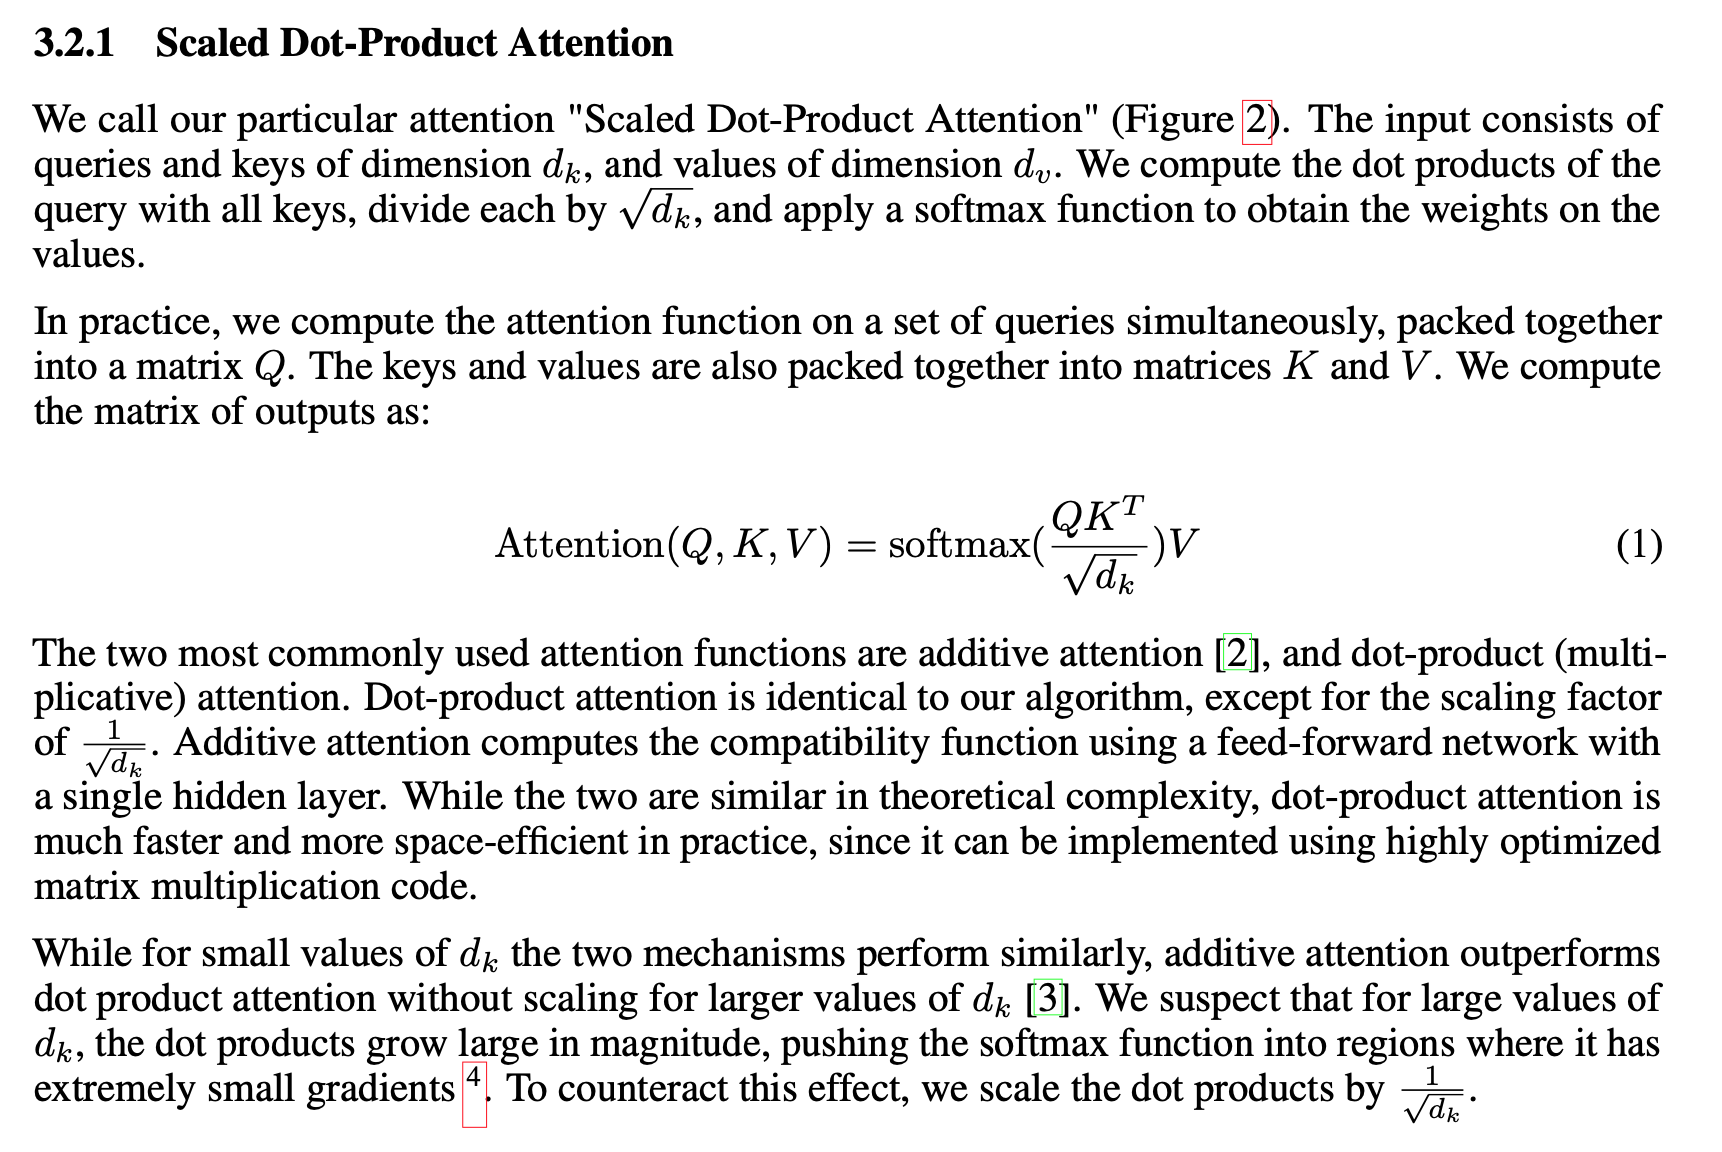
\includegraphics[scale=0.4]{1.png}
%\end{tcolorbox}

\section{Introduction}


In the context of deep learning neural networks, attention algorithms are designed for determining connections by weights between two elements in a sequential input. Self-attention was proposed by Vaswani et. al.\cite{vaswani2017attention} in 2017. A recent study\cite{crew2020google} shows that the paper written by Vaswani et. al.\cite{vaswani2017attention} was the fourth most cited paper in artificial intelligence upto 2020. In 2023, \cite{vaswani2017attention} became the second most cited paper in that original list. Self-attention mechanism has been implemented into almost all most recent LLM models. 


Suppose a sequential input $X\in \mathbb{R}^N\times \mathbb{R}^{d_x}$ is given. Denote $Q^t:=(XW_q)^t\in \mathbb{R}^{d_q}\times\mathbb{R}^{N}, K^t:=(XW_k)^t\in \mathbb{R}^{d_k}\times\mathbb{R}^{N}$, and $V^t:=(XW_v)^t\in \mathbb{R}^{d_v}\times\mathbb{R}^{N}$. The notations for denoting column vectors of each these three matrices are: $q^t_i\in \mathbb{R}^{d_q}$, $k^t_i\in \mathbb{R}^{d_k}$, and $q^v_i\in \mathbb{R}^{d_v}$. The $j$-th component of each column vector is denoted as $q^t_{ij}\in \mathbb{R}$, $k^t_{ij}\in \mathbb{R}$, and $q^v_{ij}\in \mathbb{R}$.


Now, in a standard implementation of a transformer-based model or any models that have self-attention mechanism implemented in it, $W_k, W_v,$ and $W_q$ are initiated in a way to satisfy the following four conditions:
\begin{itemize}
\item[(i)] $W_q\in\mathbb{R}^{d_x}\times\mathbb{R}^{d_q}$, $W_k\in\mathbb{R}^{d_x}\times\mathbb{R}^{d_k}$, and $W_v\in\mathbb{R}^{d_x} \times \mathbb{R}^{d_v}$,
\item[(ii)] the variance of the inner product of each column vector in $X^t$ with each column vector in either $W_q, W_k,$ or $W_v$ to be unit (all these inner products results in entries matrices: $Q^t$, $K^t$, and $V^t$),
\item[(iii)] each $q_i^t=(q_{i1},...,q_{id_q})^t$ and each $k_i^t=(k_{i1},...,k_{id_k})^t$ to be random variables with zero means, i.e. $\mathbb{E}\left( q_i^t \right) = \mathbb{E}\left(\left\lbrace q_{ij} \right\rbrace_{j=1}^{d_q}\right) =0=\mathbb{E} \left(\left\lbrace k_{ij} \right\rbrace_{j=1}^{d_k}\right)=\mathbb{E}\left( k_i^t \right), \forall i\in\left\lbrace 1,...,N\right\rbrace$, and unit variances, i.e $\text{Var}\left(q^t_i\right) =\text{Var}\left(\left\lbrace q_{ij} \right\rbrace_{j=1}^{d_q}\right) =1=\text{Var} \left(\left\lbrace k_{ij} \right\rbrace_{j=1}^{d_k}\right)=\text{Var}\left(k^t_i\right), \forall i\in\left\lbrace 1,...,N\right\rbrace$, and
\item[(iv)] $q_{i_1}^t$ and $k_{i_2}^t$ are all independent in the following ways: $\text{Cov}\left( q^t_{i_1},k^t_{i_2}\right)=0, \forall i_1,i_2,$ $\text{Cov}\left( q^t_{i_1},q^t_{i_2}\right)=0, \forall i_1\neq i_2,$, $\text{Cov}\left( k^t_{i_1},k^t_{i_2}\right)=0, \forall i_1\neq i_2.$ 
\end{itemize}
Furthermore, by convention, let $d_k=d_q$. Then, with the four above conditions satisfied, any scalar products of column vectors in $Q^t$ and $K$ have variance $d_k$ (see Appendix).

\begin{definition}
The Softmax function is defined using the Boltzmann distribution function: Given a sequential inputs (i.e. consider the finite sequence as a vector): $\left\lbrace z_i\right\rbrace, z_j\in\mathbb{R},\forall j\in\left\lbrace 1,...,n\right\rbrace$, then 
$$
\text{Softmax}(z_i) := \frac{\exp\left(z_i \right) }{\sum\limits_j \exp\left(z_j \right)}.
$$
\end{definition}

Furthermore, this distribution can be scaled by using a parameter $\beta$, and $\beta$ is the inverse of the temperature of the physical system described by the distribution:
$$
\text{Softmax}(\beta z_i) := \frac{\exp\left(\beta z_i \right) }{\sum\limits_j \exp\left(\beta z_j \right)}.
$$

In order to take inputs that are tensors, for each component of a tensor $a_{i_1i_2...i_n}$, the softmax is operated on its last dimension $i_n$, and also output a tensor which has indices $i_1...i_n$. 
For example, for a $N\times d$ tensor (i.e. a matrix), the softmax is taking on its last dimension, i.e. which equals $d$. The output is also an $N\times d$ matrix, say it is denoted by $\text{softmax}(a_{i_1i_2...i_n})_{N\times d}$. Then, each entry $\text{softmax}(a_{i_1i_2})_{ij}$ of the matrix $\text{softmax}(a_{i_1i_2})_{N\times d}$ is defined as
$$
\text{softmax}(a_{i_1i_2})_{ij}:=\frac{\exp\left(\beta a_{ij} \right) }{\sum\limits_{i_1=1}^N \exp\left(\beta a_{i_1j} \right)}.
$$
Operating on the last dimension means to fix the last index in the normalization. In this example that means to consider each column vector in $a_{i_1i_2}$ as a set of data or a physical system that Boltzmann distribution was applied to, and the result $\text{softmax}(a_{i_1i_2})_{ij}$ is the probability of the configuration $a_{ij}$. The denominator is also called the normalization factor or the partition function that it sums all possible configurations using to given data $a_{i_1i_2}$ where $i_2=j$ to be the input of the exponential function $\exp\left(\beta s \right), s\in\mathbb{R}$.

Furthermore, for a fixed $j$, the probability $\text{softmax}(a_{i_1i_2})_{ij}$ can be consider as the interaction strength between the $i$-th and $j$-th particles. 

In the following example, the self-attention mechanism, the $i$-th particle would be the column vector $q_i^t$ in the matrix $Q^t$, and the $j$-th particle would be the column vector $k^t_j$ in the matrix $K^t$.

\begin{definition}[Self-attention]
With the notations $Q,K$ and $V$, defined as above, \textit{the self-attention mechanism} is the following function
$$
\text{Attention}\left(Q,K,V\right):= \text{softmax}\left(\beta\left( QK^T \right)  \right)  V,
$$
where $\beta:=\frac{1}{\sqrt{d_k}}\in\mathbb{R}$.
\end{definition}




In self-attention, this $\beta$ is $\frac{1}{\sqrt{d_k}}$, and $T$ is the standard deviation of the scalar product $\sqrt{d_k}$.

By definition of softmax, apply softmax to the matrix $\frac{QK^T}{\sqrt{d_k}}$ means to apply Softmax function on each column of the matrix $\left(\frac{QK^T}{\sqrt{d_k}}\right)_{N\times N}$, and for defining the self-attention function, take a matrix multiplication between $\text{softmax}\left(\frac{QK^T}{\sqrt{d_k}} \right)_{N\times N}$ and the value matrix $V_{N \times d_v}$. 

\textbf{The question} that was asked and answered by this paper is the following.


Because of the random initiation of each weight matrices, if this self-attention, i.e. weights assigning process were run in parallel, then the model can learn from more than one different perspectives. In \cite{vaswani2017attention}, this notion is defined as multi-head attention. Each self-attention function  $\text{Attention}\left(Q,K,V\right)_i$ is called $\text{head}_i$, where $i$ is from 1 to $H$. The output of all $H$ heads are concatenated to a tensor denoted by $\text{Concat}\left(\text{head}_1,...,\text{head}_H \right)$, then defined $\text{Multihead(Q,K,V)}:= \text{Concat}\left(\text{head}_1,...,\text{head}_H \right) W^O$, where $W^O\in \mathbb{R}^{H\cdot d_v}\times \mathbb{R}^{d_{\text{out}}}$.


Let $\epsilon>0$ be given. Because of the mathematical form of the Boltzmann distribution, if the input is $z_i+\epsilon$, then $\text{Softmax}(\beta z_i+\epsilon)=\text{Softmax}(\beta z_i).$ However, a naive but natural question to ask is what if the scaling factor $\beta$ in Boltzmann distribution, or the self-attention function, is modified into the form $\beta^\epsilon$ or $\beta\cdot\epsilon$? It is necessary to ask this question, since we want to be able to justify why and when it makes sense to use the scaling factor $\beta=\frac{1}{\sqrt{d_k}}$ in the self-attention function. Is it sufficient to ask this question? That is the question this paper is going to answer. The next section provides a solution to this question.

However, a mathematical and statistical analysis on the question raised and answered in this paper was not found in the literature, and the issue pointed out by this paper can still be found in the most recent publications that implemented self-attention in their models.

\section{Algorithm}

To be able to make sense to use the scaling factor $\beta=\frac{1}{\sqrt{d_k}}$ in the self-attention function, the four assumptions are necessary. 

Within the four assumptions, the first assumption is usually fixed when self-attention is considered to be applied. 


Since the way query and key matrices are defined, i.e. $Q=XW_q$ and $K=XW_k$, assumption (iii) and (iv) are based on assumption (ii).

Suppose the assumptions (ii) is relaxed, the variance of the scalar product $q_ik_i$ is approximated to $\left( d_x \sigma_X^2 \sigma_{W_q}^2\right)\cdot\left(d_x \sigma_X^2 \sigma_{W_k}^2\right)\cdot d_k$. Since the training set is given, i.e. it is fixed, and so are $d_x$ and $d_k$, $\sigma_{W_q}$ and $\sigma_{W_k}$ are the actual moving factors. 

What can cause $\sigma_{W_q}$ and $\sigma_{W_k}$ to be changed? In the training phase, the gradient descent algorithm or the backpropagation is used and the algorithm is going to shift the initial probability distribution of each entry in the random matrices $W_q$ and $W_k$ to the final probability distribution at a local minimum in the moduli space (or on the loss surface).

Hence, the scaling factor $\beta=\frac{1}{\sqrt{d_k}}$ is only valid at the initial point given the four assumptions at the initial point in the moduli space, and it can hold true if the thermodynamic system described by the Boltzmann distribution is in statics, i.e. its temperature is fixed. However, since the initial point is random and unlikely to be the final point in the moduli space throughout the training mode, the assumption (ii) is not valid right after the training of the model that used self-attention function is initiated. Without assumption (ii), assumption (iii) and (iv) are invalid throughout the training and predicting modes.


To solve this problem, the solution could be written as an algorithm that it measures $\sigma_{W_q}$ and $\sigma_{W_k}$ and updates the scaling factor $\beta$ in after each iteration or batch during the training and the best scaling factor $\beta$ that is going to be used in the predicting mode could be determined by the best model chosen from the ensemble of all trained models.

This also answers the question asked in the previous section that it shows the sufficiency to ask the question.


In practice, 709 is the upper bound of the exponent of the exponential function based $e$ in lots of machines before the machines start to overflow. Likewise, on each machine, there exists a non-negative integer $N$ such that the machine starts to overflow the result. Hence, an alternative algorithm is: firstly try $ \beta \in \left\lbrace 10^N, \frac{1}{10^N} \right\rbrace$ for $N=0,1,2,...$, then run a binary search to narrow down the range of the best scaling factor $\beta$ during the training after either each iteration or batch.

A further meaning of this algorithm is shown in the next section by using an empirical example.


\section{Empirical example}

The task of the empirical example is to flip a given string of non-negative integers. In other words, the goal is to train a multihead in a transformer to learn a function that maps each index $i$ of an integer in a string to the index $(n-i)+1$ in the new string that will be returned by the model. Since the model needs to learn to swap the first and last elements in the string, it could be a challenging task for recurrent neural nets if the length of the input string is large.

In this empirical example, when the string length is 20, the range of the non-negative integers is between $0$ and $100$, and the number of samples used in training is 15000, 1000 samples for validation, and 100000 samples for testing. 

Then, without running the above alternative algorithm, i.e. when the scaling factor $\beta$ is $\frac{1}{\sqrt{d_k}}$ the validation accuracy is 1.51\%, and the test accuracy is 1.50\%. To have a stable test accuracy above 95\%, the training sample size needs to be increased from 15000 to 25000.

However, by applying the above alternative algorithm, the scaling factor is in $O(1)$, a constant $\sim 5$, with training sample size at 15000, the validation accuracy and test accuracy can already reach above 95\% stably. Thus, the above algorithms can not only compress the training set when the training samples are limited or rare, but also reduce the training time to reach the best accuracy.

Furthermore, the model that achieved the above accuracy did not achieve it by memorizing the training examples. Since a 100\% accuracy is also achievable within the ensemble, and once achieved that 100\% accuracy the model can flip any input string with the same length and the range of the values of its each word. However, if it was by memorizing, then the model had to memorize $100^{20}$ strings with length 20 which greatly exceed the number of parameters of the model (less than 8000).

The following results were obtained by restarting the training and using the following procedure:
\begin{itemize}
\item[Step 1] Start with the smallest possible amount of data and set the dynamic scaling factor to 1.
\item[Step 2] Gradually add a certain small amount of data to reach an accuracy greater than 50 percent.
\item[Step 3] Using binary search to narrow down the best possible dynamic scaling factor $\beta$.
\item[Step 4] Downsizing the training set size to the minimum with $\beta$ to be fixed.
\item[Step 5] Using the same initialization (model size, the range of the string, the string length, particularly, the training set size) but change $\beta$ from the fixed value derived from step 3 to the value suggested by the old method\cite{vaswani2017attention}, i.e. set $\beta=\frac{1}{\sqrt{d_k}}$, and record the test accuracy.
\end{itemize}

\begin{table}[H]
\begin{center}
\begin{tabular}{||c c c c c||} 
 \hline
 Methods & Input Range & String Length & Training Set Size & Test Accuracy \\ [0.5ex] 
 \hline\hline
 Old Method: $\beta=\frac{1}{\sqrt{d_k}}$  & 100 & 20 & 15000 & 1.5\% \\ 
 New Method: $\beta=5$  & 100 & 20 & 15000 & 96\% \\
 \hline
 Old Method: $\beta=\frac{1}{\sqrt{d_k}}$  & 100 & 200 & 19300 & 1.23\%\\
 New Method: $\beta=0.16$  & 100 & 200 & 19300 &  100\%\\
 \hline
 Old Method: $\beta=\frac{1}{\sqrt{d_k}}$  & 10 & 20 & 8000 &  18.56\%\\ 
 New Method: $\beta=6.55$  & 10 & 20 & 8000 &  100\%\\
 \hline
 Old Method: $\beta=\frac{1}{\sqrt{d_k}}$  & 1000 & 20 & 50000 &  18.56\%\\ 
 New Method: $\beta=5$  & 1000 & 20 & 50000 &  100\%\\
 \hline
 Old Method: $\beta=\frac{1}{\sqrt{d_k}}$  & 1000 & 20 & 40000 &  10.68\%\\ 
 New Method: $\beta=5$  & 1000 & 20 & 40000 &  99.79\%\\
 \hline
 Old Method: $\beta=\frac{1}{\sqrt{d_k}}$  & 1000 & 20 & 35000 &  5.52\%\\ 
 New Method: $\beta=5$  & 1000 & 20 & 35000 &  99.53\%\\
 New Method: $\beta=6$  & 1000 & 20 & 35000 &  99.77\%\\ [1ex] 
 \hline
 

 \hline
\end{tabular}
\caption{Let String Length $=$ Model Dimension $d_k$.  The above table is a collection of several sets of comparisons between old ($\beta=\frac{1}{\sqrt{d_k}}$) and new ($\beta$ is dynamic and derived by using a binary search) methods. The last three sets of old and new pairs showed the step 4 of the procedure for downsizing the training set to find the smallest possible training set. The last row, after reaching the smallest size of the training set, apply step 3 again to find a better $\beta$ which can increase accuracy by 0.24\%.}
\end{center}
\end{table}
\section{Discussion}

The empirical results in the previous section shows that with dynamic scaling factor being implemented, the model can reach an accuracy higher than 96\% with about half of the training data compared to the fixed scaling factor introduced in the self-attention.

Our empirical model only has one task. If it is a large model, the number of features needed to be learned by a large model such as LLMs are several orders of magnitude higher than the model that only needs to learn one task. Hence, the difference of the number of training samples needed between models that use dynamic or static scaling factor will be an exponential growth when the number of features that need to be learned grows. 
\section{Conclusion}
%\section{Limitation}

\section{Appendix: Deriving the scaling factor $\frac{1}{\sqrt{d_k}}$ used in \cite{vaswani2017attention}}


We can derive the assumption in \cite{vaswani2017attention} for the variance of $QK^T$ written in the hidden dimension $d_k$:
\begin{proposition}
Let $q_i$ and $k_i$ be random variables with zero means, i.e. $\mathbb{E} q_i=0=\mathbb{E} k_i, \forall i$, and unit variances, i.e $\text{Var} q_i=1=\text{Var}k_i$, where $i\in\left\lbrace 1,...,d_k\right\rbrace$, and they are all independent in the following ways:
$$
\text{Cov}\left( q_i,k_i\right)=0, \forall i,
$$
$$
\text{Cov}\left( q_i,q_j\right)=0, \forall i\neq j, \text{ and}
$$
$$
\text{Cov}\left( k_i,k_j\right)=0, \forall i\neq j.
$$
Then
$$
\text{Var}\left( QK^T\right)=d_k.
$$
\end{proposition}
 
\begin{proof}
$$
\text{Var}\left( QK^T\right)
$$
$$
=\text{Var}\left( \sum\limits_{i=1}^{d_k}q_ik_i\right)
$$
$$
=\sum\limits_i \text{Var}\left( q_ik_i\right)
$$
$$
=\sum\limits_i \text{Var}\left( q_i\right) \text{Var}\left( k_i\right)
$$
$$
=\sum\limits_i 1\cdot 1
$$
$$
=d_k.
$$
\end{proof}
The first equality is because in \cite{vaswani2017attention}, $Q$ and $K$ are row vectors, and $QK^T$ is taking their scalar product. The second equality is because $\text{Cov}\left( q_i,q_j\right)=0, \forall i\neq j, \text{ and } \text{Cov}\left( k_i,k_j\right)=0, \forall i\neq j.$ Then, the variance of the sum is the sum of variances. The third equality is because of the conditions $\mathbb{E} q_i=0=\mathbb{E} k_i, \forall i$ and $\text{Cov}\left( q_i,k_i\right)=0, \forall i$, hence we have the variance of the product is the product of variances.

The authors in \cite{vaswani2017attention} want to scale the result of $QK^T$ using the standard deviation of the scalar product, so $QK^T$ is multiplied by a factor 
$$\frac{1}{\sqrt{\text{Var}\left(QK^T \right)}}=\frac{1}{\sqrt{d_k}}.$$


%\begin{lstlisting}[language=iPython]
%<- #there shouldn't be quotation marks
%"""
%---------
%sin2_theta  = np.sin(theta)**2 - a + b
%"""
%import math
%import numpy as np
%from lib.analytical import csa
%MAS = math.degrees(math.acos(math.sqrt(1/3)))/360 * 2* math.pi + a -b
%\end{lstlisting}

\bibliographystyle{amsplain} % We choose the "plain" reference style
\bibliography{refs} % Entries are in the refs.bib file
\end{document}




